\documentclass[herrin-thesis.tex]{subfiles}
\begin{document}

\chapter{Neutrinos}
\label{ch:neutrinos}

\section{History}
\subsection{Beta Decay}
Neutrino physics first arose in the study of beta decay. In the most basic form of beta decay, a neutron in the nucleus decays to a proton and emits an electron. \todo{Who first found a continuous spectrum for the electron?}Early nuclear physicists discovered that unlike alpha particles and gamma rays, which are emitted in monoenergetic lines from nuclear processes, beta decay electrons were emitted with a continuous range of energies. Rather than abandoning the principle of energy conservation, Wolfgang Pauli\addref in 1930 proposed a massless particle that could carry away the ``missing energy'' in beta decays. In 1933, Enrico Fermi\addref combined the idea with Heisenberg's nucleon model to form a theory of beta decay.

\subsection{Discovery}
For several decades after Pauli proposed the neutrino, the only evidence for its existence was indirect, through momentum and energy conservation. It was not until 1956 that Cowan and Reines\addref observed the electron antineutrino. Their experiment consisted of a large tank of water with cadmium chloride dissolved. Electron antineutrinos from a nearby nuclear reactor would interact with protons in the water molecules, creating a positron and a neutron. In the experiment, the positron annihilated, producing gamma rays. Cadmium is a good neutron absorbed, and the capture created another gamma ray. The delayed coincidence of the two gamma rays provided evidence of inverse beta decay.

The discovery of the muon in 1936 provided the possibility of a muon neutrino, distinct from the electron neutrino. In 1962, Lederman, Schwartz, and Steinberger\addref showed that a beam of neutrinos, created from a beam of decaying pions, aways interacted to form muons and not electrons. We now know that each charged lepton forms an isospin doublet with its associated neutrino.

\section{The Nature of Neutrinos}
\section{Dirac Particles}
In the standard model of particle physics, neutrinos are massless and left-handed, forming an SU(2) doublet with the left-handed charged leptons. The right-handed charged leptons form an SU(2) singlet. The mass of a changed lepton is generated by a Yukawa coupling between the left-handed lepton, the right-handed lepton, and the Higgs field. Since neutrinos have been observed to have mass, then, it seems natural to generate their mass in an analogous way. This would introduce right-handed neutrinos (and left-handed antineutrinos) that would not interact weakly. However, given the observed smallness of neutrino masses, this requires Yukawa couplings much, much smaller than those of charged leptons and quarks.

\subsection{Majorana Particles}
Neutrinos do not carry charge, and so mass terms of the form
\begin{equation}
\mathcal{L}_{m}^{\nu} = -\frac{1}{2}\overline{\nu_{L}} m_{L L}^{\nu} \nu_{L}^{c} +h.c.
\label{eq:nu_majorana_lagrangian}
\end{equation}
can be added to the standard model Lagrangian. Such terms are not allowed for charge leptons, since they would violate electric charge conservation. Total lepton number conservation is an accidental symmetry in the standard model, and so it is not troublesome that these terms violate it. The particles associated with fields with such mass terms are known as Majorana particles.

Mass terms like those in \cref{eq:nu_majorana_lagrangian} can arise from many different phenomena. Without introducing new particles, S.~Weinberg\cite{Weinberg:1979qa} proposed such terms with Yukawa couplings suppressed by Planck-scale masses. However, this leads to neutrino masses that are smaller than the observed mass splittings and so is presently disfavored. Once again introducing right-handed neutrinos provides another mechanism. With right-handed neutrinos, the the most general way to write the mass terms for one generation is 
\begin{equation}
\mathcal{L}_{m}^{\nu} = -\frac{1}{2}
\begin{pmatrix}
	\overline{\nu_{L}} 	&	\overline{\nu_{R}^{c}}
\end{pmatrix}
\begin{pmatrix}
	m_{L L} 		&	m_{L R}			\\
	m_{L R}		&	M_{R R}
\end{pmatrix}
\begin{pmatrix}
	\nu_{L}^{c}	\\
	\nu_{R}
\end{pmatrix} + h.c.
\label{eq:nu_mass_matrix}
\end{equation}
where \(m_{L R}\) is a dirac mass and \(m_{L L}\) and \(M_{R R}\) are Majorana masses. Diagonalizing this yields two mass eigenstates:
\begin{equation}
m_{\pm} = \frac{1}{2}\left | (M_{R R} + m_{L L}) \pm \sqrt{\left(M_{R R} - m_{L L}\right)^2 + 4 m_{L R}^2}\right |
\label{eq:nu_diagonalized_masses}
\end{equation}
The case in which \(m_{L L} = 0\) and \(M_{R R}\gg m_{L R}\) is known as a type I seesaw mechanism. In this case, \(m_{-} \approx m_{L R}^2/M_{R R}\) and \(m_{+} \approx M_{R R}\). It is so-named because for \(m_{L R}\) on the order of quark or charged lepton masses, \(M_{R R}\) much greater than the electroweak scale levers the light neutrino masses (\(m_{-}\)) to very small values. The light neutrinos are a mixture of left and right-handed neutrinos, but the right-handed amplitude is suppressed by \(m_{L R}/M_{R R}\) and so is negligible.

\subsection{Majorons}


\section{Neutrino Mixing and Oscillation}
Neutrino mixing is described by the unitary Pontecorco-Maki-Nakagawa-Sakata (PMNS) matrix \(U\). In the case of three mass eigenstates and 3 flavor eigenstates, \(U\) can be parameterized by three Euler rotation angles, one Dirac CP violation phase, and two Majorana CP violation phases (is the neutrino is a Majorana particle):
\begin{align}
U =&\begin{pmatrix}
	U_{e1}	&	U_{e2}	& 	U_{e3}	\\
	U_{\mu1}	&	U_{\mu2}	& 	U_{\mu3}	\\
	U_{\tau1}	&	U_{\tau2}	& 	U_{\tau3}	\\
	\end{pmatrix}\\
%     =&\begin{pmatrix}
%	1	&	0		&	0		\\
%	0	&	c_{23}	&	s_{23}	\\
%	0	&	-s_{23}	&	c_{23}	\\
%	\end{pmatrix}
%	\begin{pmatrix}
%	c_{13}			&	0	&	s_{13}e^{-i\delta}	\\
%	0				&	1	&	0				\\
%	-s_{13}e^{i\delta}	&	0	&	c_{13}			\\
%	\end{pmatrix}
%	\begin{pmatrix}
%	c_{12}	&	s_{12}	&	0	\\
%	-s_{12}	&	c_{12}	&	0	\\
%	0		&	0		&	1	\\
%	\end{pmatrix}
	=&\begin{pmatrix}
	c_{12}c_{13}							&	s_{12}c_{13}							&	s_{13}e^{-i\delta}	\\
	-s_{12}c_{23}-c_{12}s_{23}s_{13}e^{i\delta}	&	c_{12}c_{23}-s_{12}s_{23}s_{13}e^{i\delta}	&	s_{23}c_{13}		\\
	s_{12}s_{23}-c_{12}c_{23}s_{13}e^{i\delta}	&	-c_{12}s_{23}-s_{12}c_{23}s_{13}e^{i\delta}	&	c_{23}c_{13}
	\end{pmatrix}
	\begin{pmatrix}
	1	&	0					&	0	\\
	0	&	e^{\frac{i\alpha_{21}}{2}}	&	0	\\
	0	&	0					&	e^{\frac{i\alpha_{31}}{2}}
	\end{pmatrix}\nonumber
\label{eq:nu_pmns_matrix}
\end{align}
where the \(s_{ij}\) denote \(\sin\theta_{ij}\) and \(c_{ij}\) denote \(\cos\theta_{ij}\). \(\delta\) is the Dirac CP violation phase, and \(\alpha_{21}\) and \(\alpha_{31}\) are the Majorana CP violation phases.

 A flavor eigenstate, such as a neutrino produced by the decay of a lepton, is a superposition of mass eigenstates:
 \begin{equation}
 \Ket{\nu_{\ell}} = \sum_{i}U_{\ell i}^{*} \Ket{\nu_i}
 \label{eq:nu_superposition}
 \end{equation}
 This mixing is illustrated in \cref{fig:nu_mixing}.
 
 The time evolution of a mass eigenstate is simply
 \begin{equation}
 \Ket{\nu_{i}(t)} = e^{-i(E_i t - \vec{p}_i\cdot\vec{x})}\Ket{\nu_i(0)}
 \label{eq:nu_time_evolution}
 \end{equation}

Neutrinos have such small masses that they are always observed in a hyper-relativistic state, in which \(t\approx L\), \(p\approx E\), where \(E\) is the total energy of the neutrino. In this limit, the phase in the exponent for \cref{eq:nu_time_evolution} becomes \(m_i^2 L/(2E)\). Combining this and \cref{eq:nu_superposition}, then the probability for a neutrino with flavor \(\alpha\) and energy \(E\) to oscillate to a neutrino with flavor \(\beta\) after traveling distance \(L\) is
\begin{align}
P_{\alpha\rightarrow\beta}	& = \left | \Braket{\nu_\beta | \nu_\alpha(L)} \right |	& = \delta_{\alpha\beta}	& - 4\sum_{i>j}\text{Re}\left(U_{\alpha i}^{*}U_{\beta i}U_{\alpha j}U_{\beta j}^{*}\right)\sin^2\left(\frac{\Delta m_{ij}^2 L}{4 E}\right)\nonumber\\
						&										&					& +2\sum_{i>j}\text{Im}\left(U_{\alpha i}^{*}U_{\beta i}U_{\alpha j}U_{\beta j}^{*}\right)\sin^2\left(\frac{\Delta m_{ij}^2 L}{2 E}\right)
\label{eq:nu_oscillation_prob}
\end{align}
Thus, the probability depends only on the angles in the mixing matrix \(U\), the difference between the squares of the masses \(\Delta m_{ij}^2\), and the ratio of distance travelled to neutrino energy \(L/E\). If there is no CP violation, \(U\) is real and the second sum is zero. Since the Majorana phases only enter \(U\) as a diagonal factor, they do not affect the oscillation probability, and thus oscillation experiments cannot determine the Majorana nature of the neutrino.

\section{Massive Neutrino Physics}

\section{Measuring Neutrino Masses}

\begin{figure}
	\centering
	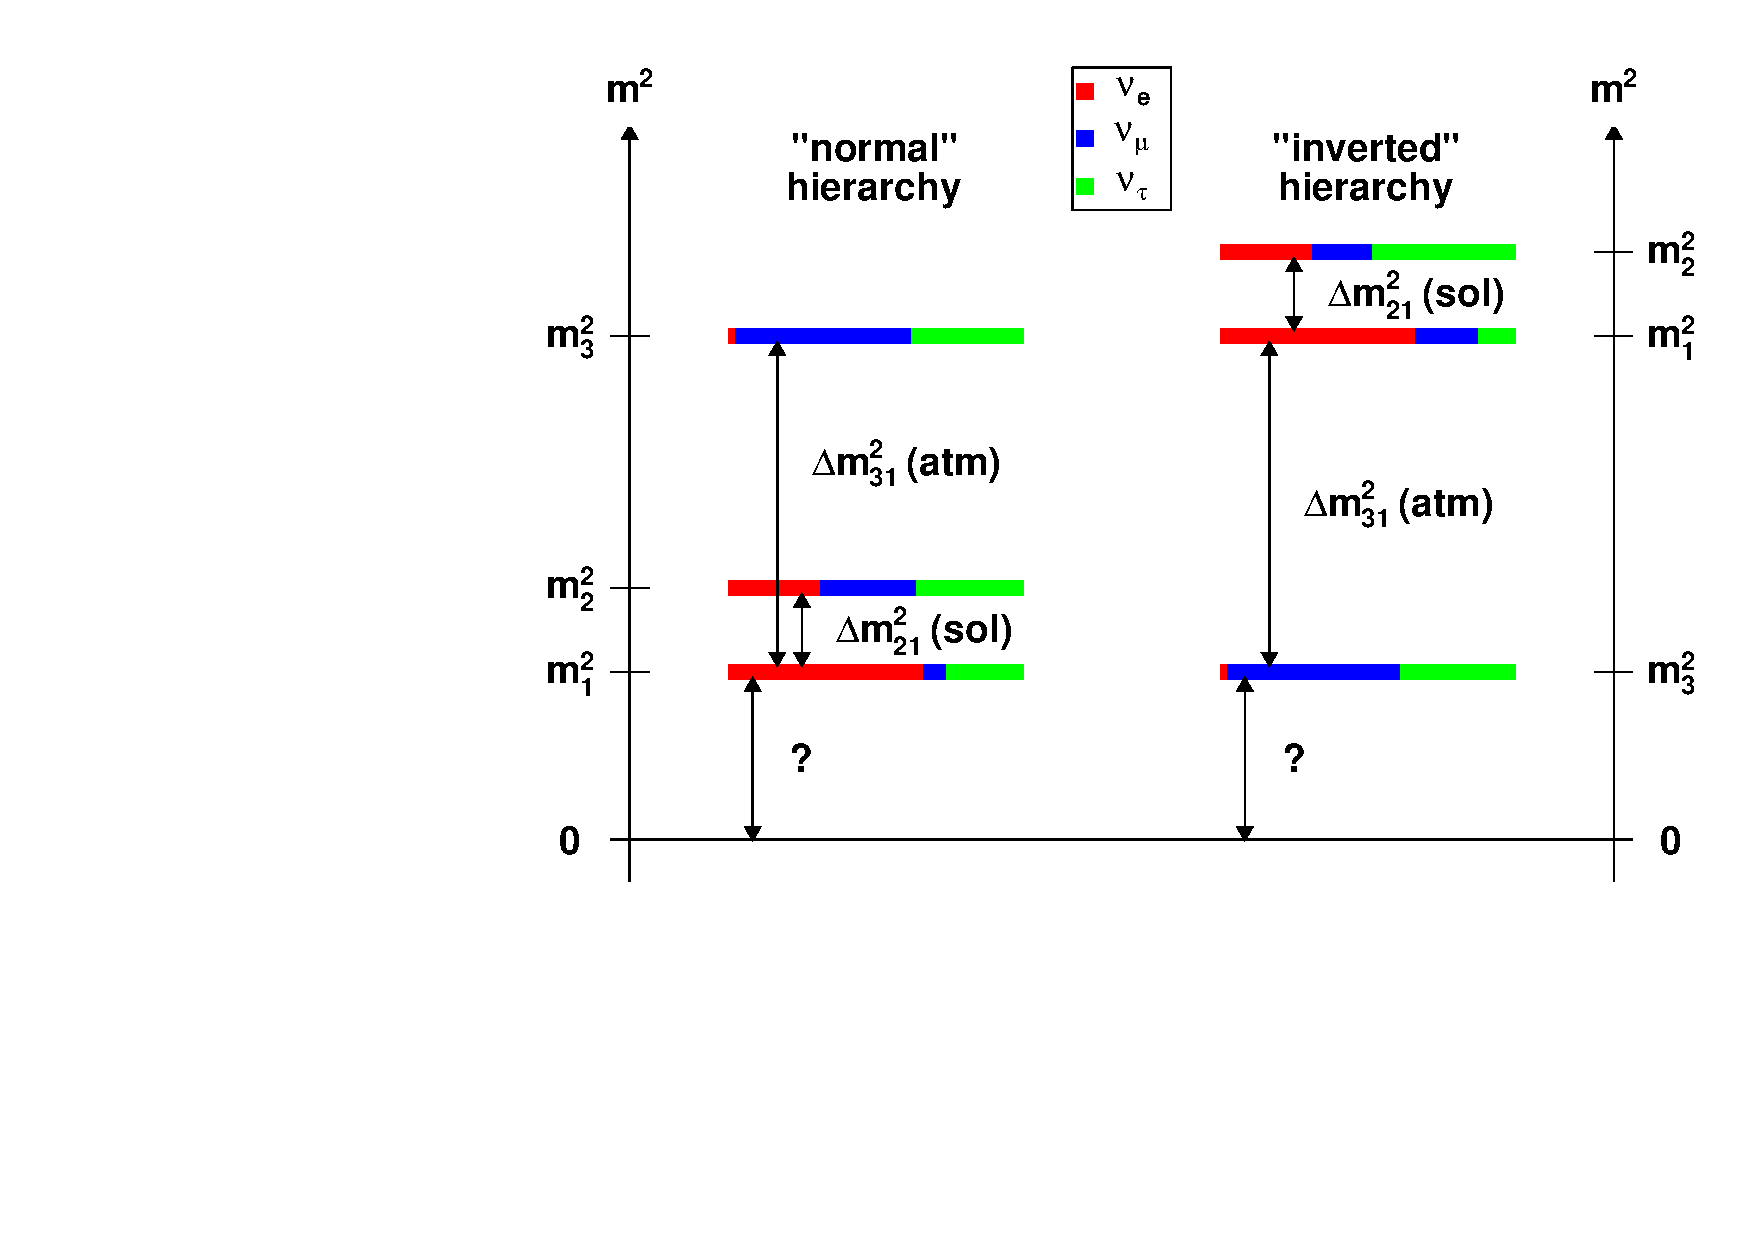
\includegraphics[width=0.6\textwidth]{./plots/nu_mixing.pdf}
	\caption[Neutrino mixing]{The neutrino mass eigenstates (represented by the horizontal bands) are each a mixture of the flavor eigenstates (represented by the different colors). The mixing angles in the PMNS matrix provide the flavor compositions of each mass state. The splittings between the squares of the masses of the mass eigenstates are known (but not shown to scale), though the sign of \(\Delta m_{31}^2\) remains unknown, allowing for the possibility of an ``inverted'' mass hierarchy. The absolute scale of the neutrino masses is also unknown.}
	\label{fig:nu_mixing}
\end{figure}

Neutrinos are observed to oscillate, and thus according to \cref{eq:nu_oscillation_prob}, the mass-squared splittings have been measured to be nonzero. The sign of \(\Delta m_{21}\) is known from the effect of matter on neutrinos emitted by the sun (known as the MSW effect), while only the magnitude of \(\Delta m_{31}\) is known. The mass splittings provide a weak lower bounds on the masses of two mass eigenstates. This does not determine the absolute mass scale, however, and the lightest eigenstate may have zero mass. If also does not determine which mass eigenstate is the lightest. \Cref{fig:nu_mixing} summarizes the situation. Other experiments, described below, may be able to measure the absolute mass scale and possibly determine the hierarchy of the mass eigenstates. However, to date, they have only provided upper bounds on the mass.

\subsection{Beta Decay Endpoint}
\begin{figure}
	\centering
	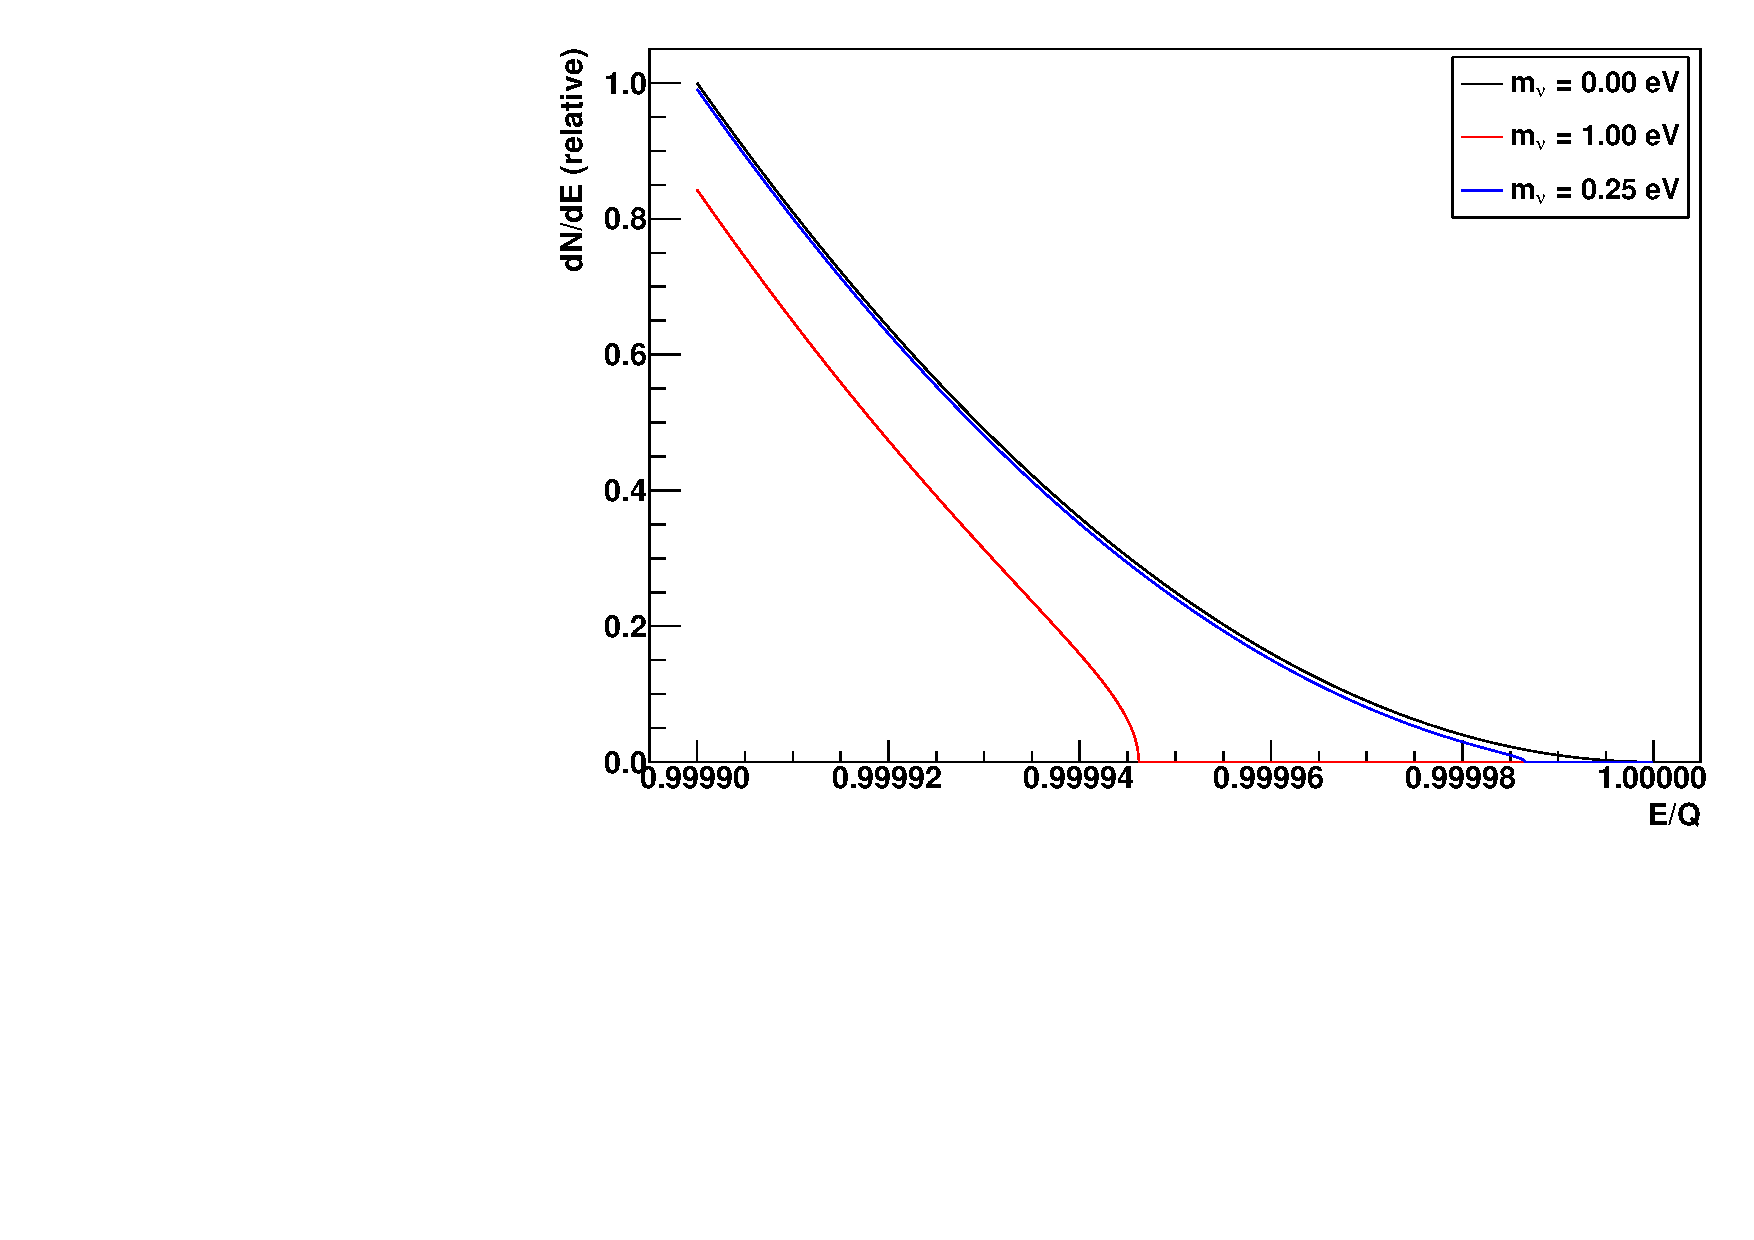
\includegraphics[width=0.6\textwidth]{./plots/nu_beta_endpt.pdf}
	\caption[Beta decay spectrum endpoint for massive neutrinos]{The endpoint of the electron energy spectrum for beta decay for several neutrino masses. Experiments like Mainz and KATRIN aim to measure the neutrino mass by looking for the slight distortion of the spectrum close to the Q value of the decay due to the neutrino mass.}
	\label{fig:nu_beta_endpt}
\end{figure}

When an isotope beta decays, it emits an electron-antineutrino which carries away some energy from the decay. However, this amount may be very small, and so in rare cases, the electron may cary away nearly all of the energy of the decay. A neutrino with nonzero rest mass will always take some energy to create, however, limiting the maximum energy of the electron and distorting the spectrum. This is illustrated in \cref{fig:nu_beta_endpt}.

An experiment looking at the beta decay spectrum will measure the effective mass squared of the electron neutrino:
\begin{equation}
m^2\left(\nu_e\right) = \sum_j \left | U_{e j} \right |^2 m^2\left(\nu_j\right)
\label{eq:nu_beta_endpt_mass}
\end{equation}
The best limits come from the Mainz and Troitsk experiments, which examined the spectrum of tritium. Mainz measured \(m(\nu_e) \leq 2.3 \text{ eV}/\text{c}^{2}\)\cite{Kraus:2005nx}, while Troitsk measured \(m(\nu_e) \leq 2.05 \text{ eV}/\text{c}^{2}\)\cite{Aseev:2011dq}, both at the 95\% confidence level. The KATRIN experiment, which will begin operation soon and also examine the spectrum for tritium, hopes to be sensitive to masses greater than \(200\text{ meV}/\text{c}^2\)\cite{Osipowicz:2001oq}.

\subsection{Cosmology}
Due to their small masses, neutrinos in the early universe did not clump together like most other matter. The distribution of matter in the universe, then, is sensitive to the mass ratio of neutrinos to other matter. Thus, cosmological surveys of structure and anisotropy can potentially measure \(\sum m_{\nu}\). Cosmic microwave background data from the Planck satellite provide the best limit to date. The Planck data yield \(\sum m_{\nu} < (0.23 - 1.08) \text{ eV}/\text{c}^2\), with the spread depending on which other data sets are used\cite{Ade:2013kl}. Further data from other surveys may push the sensitivity down to the \si{\eV} scale\cite{Abazajian:2011tg}.

\subsection{Double Beta Decay}

\begin{figure}
	\centering
	\begin{subfigure}[b]{0.48\textwidth}
		\centering
		\includegraphics[width=\textwidth]{./feynman_diagrams/twonubetabeta.pdf}
		\caption[Diagram of \(2\nu\beta\beta\)]{The standard model allowed mode of two neutrino double beta decay.}
		\label{fig:diagram_2nubb}
	\end{subfigure}\hfill%
         \begin{subfigure}[b]{0.48\textwidth}
		\centering
		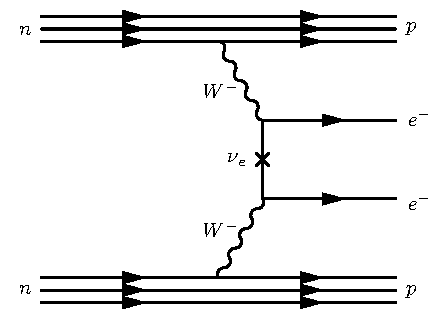
\includegraphics[width=\textwidth]{./feynman_diagrams/zeronubetabeta.pdf}
		\caption[Diagram of \(0\nu\beta\beta\)]{The neutrinoless mode of double beta decay.}
		\label{fig:diagram_0nubb}
	\end{subfigure}
	\label{fig:diagrams}
	\caption[Double beta decay modes]{Double beta decay modes}
\end{figure}

Double beta decay (\twonu)is a standard model process in which two neutrons simultaneously decay to two protons, emitting two electrons and two antineutrinos. \Cref{fig:diagram_2nubb} illustrates this process. It has been observed in a number of isotopes with half lives between \SI{7.1d18}{\year} for \isotope{100}{Mo}\cite{Arnold:2005hc} and \SI{2.2d21}{\year} for \xenon{136}\cite{Auger:2012ar}.

If neutrinos are Majorana particles, then there is the potential to observe neutrinoless double beta decay (\zeronu). The simplest mechanism, shown in \cref{fig:diagram_0nubb}, has a light Majorana neutrino being exchanged. In this process two electrons are emitted, but unlike \twonu, the electrons carry away the entire energy of the decay. Thus, this decay mode should be observable in a detector with good energy resolution. \Cref{fig:nu_twonu_zeronu_comparison} illustrates the the difference in the sum electron spectrum for the two modes. If \zeronu does indeed proceed through light neutrino exchange, then the rate is given by
\begin{equation}
\left [ T^{0\nu}_{1/2} \right ]^{-1} = G^{0\nu}\left(E, Z\right)\frac{\left | \langle m_{\beta\beta} \rangle \right |^2}{m_e^2}\left | \mathcal{M}^{0\nu}\right |^2
\label{eq:nu_zeronu_rate}
\end{equation}
where \(G^{0\nu}(E,Z)\) is a calculable phase-space factor, \(m_e\) is the mass of the electron, \( \mathcal{M}^{0\nu}\) is the nuclear matrix element, which can be estimated with models, and
\begin{equation}
\langle m_{\beta\beta} \rangle = \sum_i U_{e i}^2 m_i
\label{eq:nu_meff_def}
\end{equation}
is known as the ``effective mass''. A number of experiments have attempted to look for neutrinoless double beta decay, but it has not yet been observed. A controversial claim by a subset of the Heidelberg-Moscow collaboration report discovery of \zeronu in \isotope{76}{Ge}\cite{KlapdorKleingrothaus:2006ff}, but this is in tension with results from \isotope{136}{Xe} experiments\cite{Auger:2012ar}\cite{Gando:2013fk}. \Cref{tab:nu_zeronu_limits} summarizes the present status of experiments.

\begin{table}[htd]
\centering
\caption[Current \zeronu limits]{Results of searches for neutrinoless double beta decay. Effective masses limits are as reported by the experiments, and no attempt has been made to standardize the nuclear matrix element calculation used. Where a range has been reported, it is due to variation between different nuclear matrix element calculations.}
\label{tab:nu_zeronu_limits}
\begin{tabular}{c c c c}\toprule
	isotope			&	half-life (\(\times10^{22}\) \si{\year})	&	\(\left|\langle m_{\beta\beta}\rangle\right |\) (\si{\eV})	&	experiment	\\\midrule
	\isotope{48}{Ca}	&	\(>5.8\)						&	\(< (3.5-22)\)								& 	\ce{CaF2(Eu)} scintillators\cite{Umehara:2008ij}\\
	\isotope{76}{Ge}	&	\(>1900\)						&	\(< 0.35\)									&	Heidelberg-Moscow\cite{Klapdor-Kleingrothaus:2001bs}\\
	\isotope{76}{Ge}	&	\(2230^{+440}_{-310}\)			&	\(0.32\pm0.03\)								&	Subset of H-M\cite{KlapdorKleingrothaus:2006ff}\\
	\isotope{82}{Se}	&	\(>36\)						&	\(< (0.89 - 2.43)\)							&	NEMO-3\cite{Barabash:2011fv}\\
	\isotope{96}{Zr}		&	\(>0.92\)						&	\(< (7.2 - 19.5)\)								&	NEMO-3\cite{Barabash:2011fv}\\
	\isotope{100}{Mo}	&	\(>110\)						&	\(< (0.45 - 0.93)\)							&	NEMO-3\cite{Barabash:2011fv}\\
	\isotope{116}{Cd}	&	\(>17\)						&	\(< 1.7\)									&	Solotvina\cite{Danevich:2003dz}\\
	\isotope{130}{Te}	&	\(>280\)						&	\(< (0.30 - 0.71)\)								&	CUORICINO\cite{Andreotti:2011fu}\\
	\isotope{136}{Xe}	&	\(>1600\)						&	\(< (0.14 - 	0.38)\)							&	EXO-200\cite{Auger:2012ar}\\
	\isotope{136}{Xe}	&	\(>1900\)						&	\(< (0.13 - 	0.35)\)							&	KamLAND-Zen\cite{Gando:2013fk}\\
	\isotope{150}{Nd}	&	\(>1.8\)						&	\( < (4.0 - 6.3)\)								&	NEMO-3\cite{Barabash:2011fv}\\\bottomrule
\end{tabular}
\end{table}

\subsection{Summary}

\begin{figure}
	\centering
	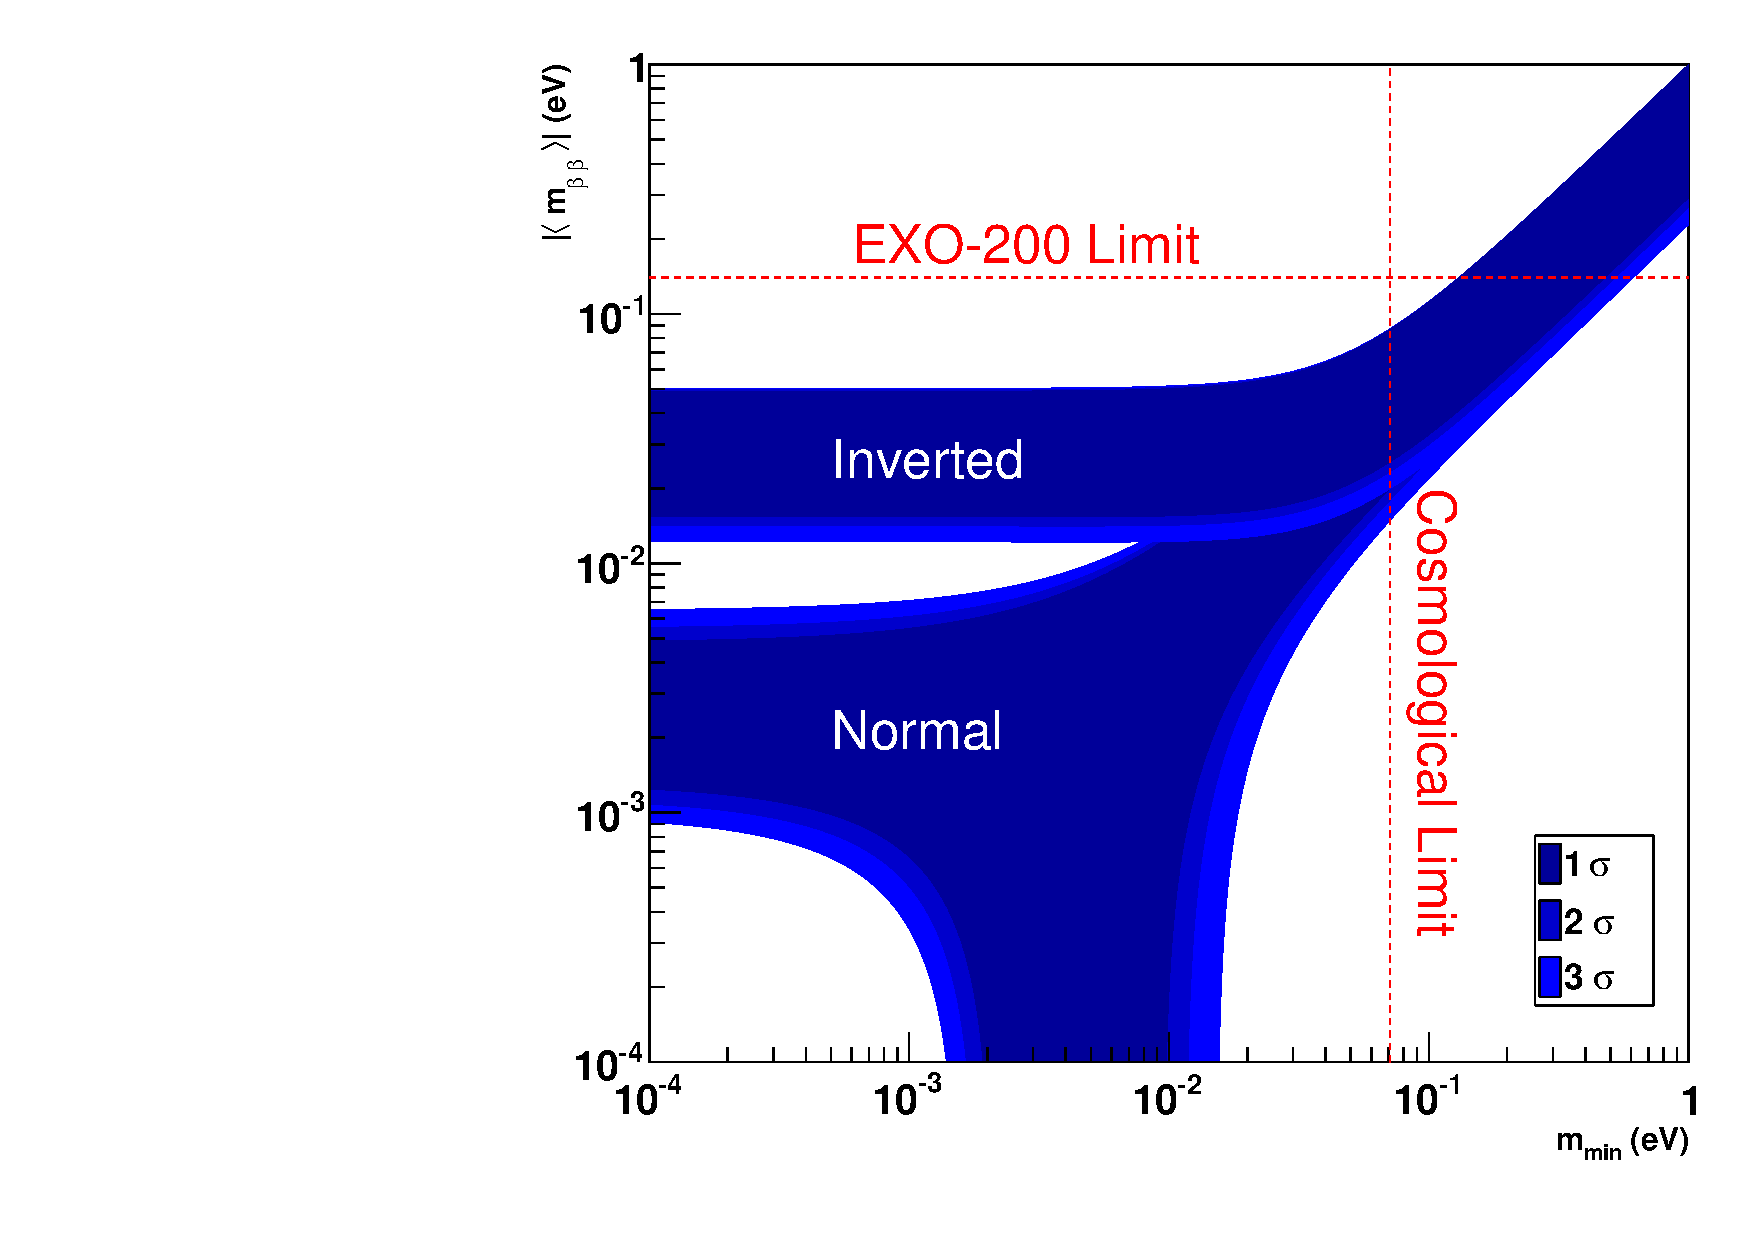
\includegraphics[width=0.6\textwidth]{./plots/nu_meff_v_mmin.pdf}
	\caption[Effective Majorana mass vs. smallest neutrino mass]{The allowed values for the effective Majorana mass as a function of the smallest neutrino mass for both the inverted and normal mass hierarchies. The widths of the bands depend on the Majorana phases. Uncertainties on the mixing angles and mass splittings widen these bands.The mixing angles, mass splittings, and uncertainties used are from a global fit by Forero et al.\cite{Forero:2012cr} The cosmological limit comes from the Planck satellite. Constraints on the sum of the neutrino masses combined with the mass splittings yield an upper bound for the smallest neutrino mass.}
	\label{fig:nu_meff_v_mmin}
\end{figure}\addref



\end{document}
